\documentclass{standalone}

\usepackage{tikz}

\usepackage{graphicx}
\usetikzlibrary{angles, quotes}
	\usetikzlibrary{arrows.meta, positioning, quotes, shapes, shapes.geometric}
	\definecolor{baseline6}{HTML}{6940FF}
	\definecolor{baseline5}{HTML}{A12EFF}
	\definecolor{baseline4}{HTML}{D24AFF}
	\definecolor{baseline3}{HTML}{FF7DF0}
	\definecolor{baseline2}{HTML}{FFBDD4}
	
	\definecolor{thick6}{HTML}{00BDA8}
	\definecolor{thick2}{HTML}{77F3DB}
	
	\definecolor{thin6}{HTML}{D47E04}
	\definecolor{thin2}{HTML}{FFDA09}
	
	\definecolor{single}{HTML}{00A2FF}
	\definecolor{full}{HTML}{425df5}
	
	\definecolor{expt1col}{HTML}{FF0099}
	\definecolor{expt3col}{HTML}{527319}
	\definecolor{expt2col}{HTML}{0000FF}
	\tikzset{nodes={font=\sffamily}} 
	\tikzset{
		axis/.style={nodes={font=\sffamily\bfseries}},
		expt1/.style={
			draw, circle, color=expt1col, line width=0, align=center, scale=1.5, font=\sffamily},
		expt2/.style={
			draw, circle, color=expt2col, line width=0,  align=center, scale=1.5, font=\sffamily},
		expt3/.style={
			draw, circle, color=expt3col, line width=0, align=center, scale=1.5, font=\sffamily},
		illus/.style={draw, rectangle, align=center},
		annotate/.style={
			color=black!60, line width=0, align=center, scale=1, font=\sffamily},
		illus/.style={draw, rectangle, align=center, color=black!50, font=\sffamily, scale=1},
		bound/.style={draw, rectangle, align=center, color=black, font=\sffamily, scale=1}
	}
	
\begin{document}
\begin{tikzpicture}
		
		\node at (-4.5,5.5) {\LARGE\bfseries{A}};

	%	\node at (13,4) {\LARGE\bfseries{C}};

		\def\r{4}
		\def\t{3}
		\draw (0,0) edge[-Stealth, line width=1] [axis, "Listener Backchannel", sloped, pos=.55, inner sep=2ex] (-\r/1.4,  -\r/1.4) ;
		\draw (0,0) edge[-Stealth, line width=1] [axis, "Group Size", pos=1.05] (\r, 0) ;
		\draw (0,0) edge[-Stealth, line width=1] [axis, "Group coherence", sloped, pos=.45, inner sep=1.5ex] (0, \r);
		\draw[dashed] (\t,0) edge [] (\t-\t/1.4, -\t/1.4);
		\draw[dashed] (-\t/1.4,-\t/1.4) edge [] (\t-\t/1.4, -\t/1.4);
		\draw[dashed] (0,\t) edge [] (\t,\t);
		\draw[dashed] (\t,0) edge [] (\t+.2,\t/2-.2);
		\draw[dashed] (\t,0) edge [] (\t-.2,\t/2+.2);
		\draw[dashed] (\t,\t) edge [] (\t+.2,\t/2-.2);
		\draw[dashed] (\t,\t) edge [] (\t-.2,\t/2+.2);
		
		\node (n2) at (0,0) [expt1, fill=baseline2, label={[expt1col]below:2}] {};
		\node (n3) at (\t/4,0) [expt1, fill=baseline3, label={[expt1col]below:3}] {};
		\node (n4) at (\t/2,0) [expt1, fill=baseline4, label={[expt1col]below:4}] {};
		\node (n5) at (3*\t/4,0) [expt1, fill=baseline5, label={[expt1col]below:5}] {};
		\node (n6) at (\t,0) [expt1, fill=baseline6] {};
		\node[align=center,anchor=north,text=expt1col] at (\t*1.1,-.45) {6 baseline};
		
		\node (n2thick) at (0,\t) [expt3, fill=thick2, label= {[expt3col]above right:2 thick}] {};
		\node (n6thick) at (\t,\t) [expt3, fill=thick6, label={[expt3col]right:6 thick}] {};
		
		\node (nfull) at (\t+.2,\t/2-.2) [expt2, fill=full, label={[expt2col, align=center] right :6 full \\feedback}] {};
		\node (nsingle) at (\t-.2,\t/2+.2) [expt2, fill=single, label={[expt2col, align=center ]above right :6 consistent\\ speaker}] {};
		
		\node (n2thin) at (-\t/1.4, -\t/1.4) [expt3, fill=thin2, label={[expt3col]below right: 2 thin}] {};
		\node (n6thin2) at (\t-\t/1.4+.1, -\t/1.4+.1)[expt2, fill=thin6, label={[expt2col] right: 6 thin}] {};
		\node (n6thin) at (\t-\t/1.4-.1, -\t/1.4-.1) [expt3, fill=thin6, label={[expt3col]below right: 6 thin}] {};
		
		\node[annotate, anchor=north] (lab1) at (-2,2) {Rotating speaker;\\limited feedback};
		\node[annotate,anchor=north] (lab2) at (-1.1,4.5) {Consistent speaker;\\full feedback};
		\node[annotate,anchor=north] (lab3) at (-2,0.8) {Listeners \\use chat};
		\node[annotate,anchor=north] (lab4) at (-1.5,-3) {Listeners \\use emoji};
		
		\node[align=center,anchor=north, text=expt1col] (ex1) at (1.2,2.5) {Experiment 1};
		\node[align=center,anchor=north, text=expt2col] (ex1) at (1.2,2) {Experiment 2};
		\node[align=center,anchor=north, text=expt3col] (ex1) at (1.2,1.5) {Experiment 3};
			\begin{scope}[line width=1 pt, >=Stealth, color=black!60]
			\draw[->] (lab1) -> (n2);
			\draw[->] (lab2) -> (n2thick);
			\draw[->] (lab3) -> (n2);
			\draw[->] (lab4) -> (n2thin);
			
		\end{scope}
		%	\node[bound, ultra thick, anchor=north west, minimum width=28em, minimum height=28em] (block) at (-4, 5) {};

		\node at (6.5,5.5) {\LARGE\bfseries{B}};
	%	\node[bound, ultra thick, anchor=north west, minimum width=28em, minimum height=28em] (block) at (7, 5) {};
		\node[illus, anchor=north west] () at (8.3, 2.3) {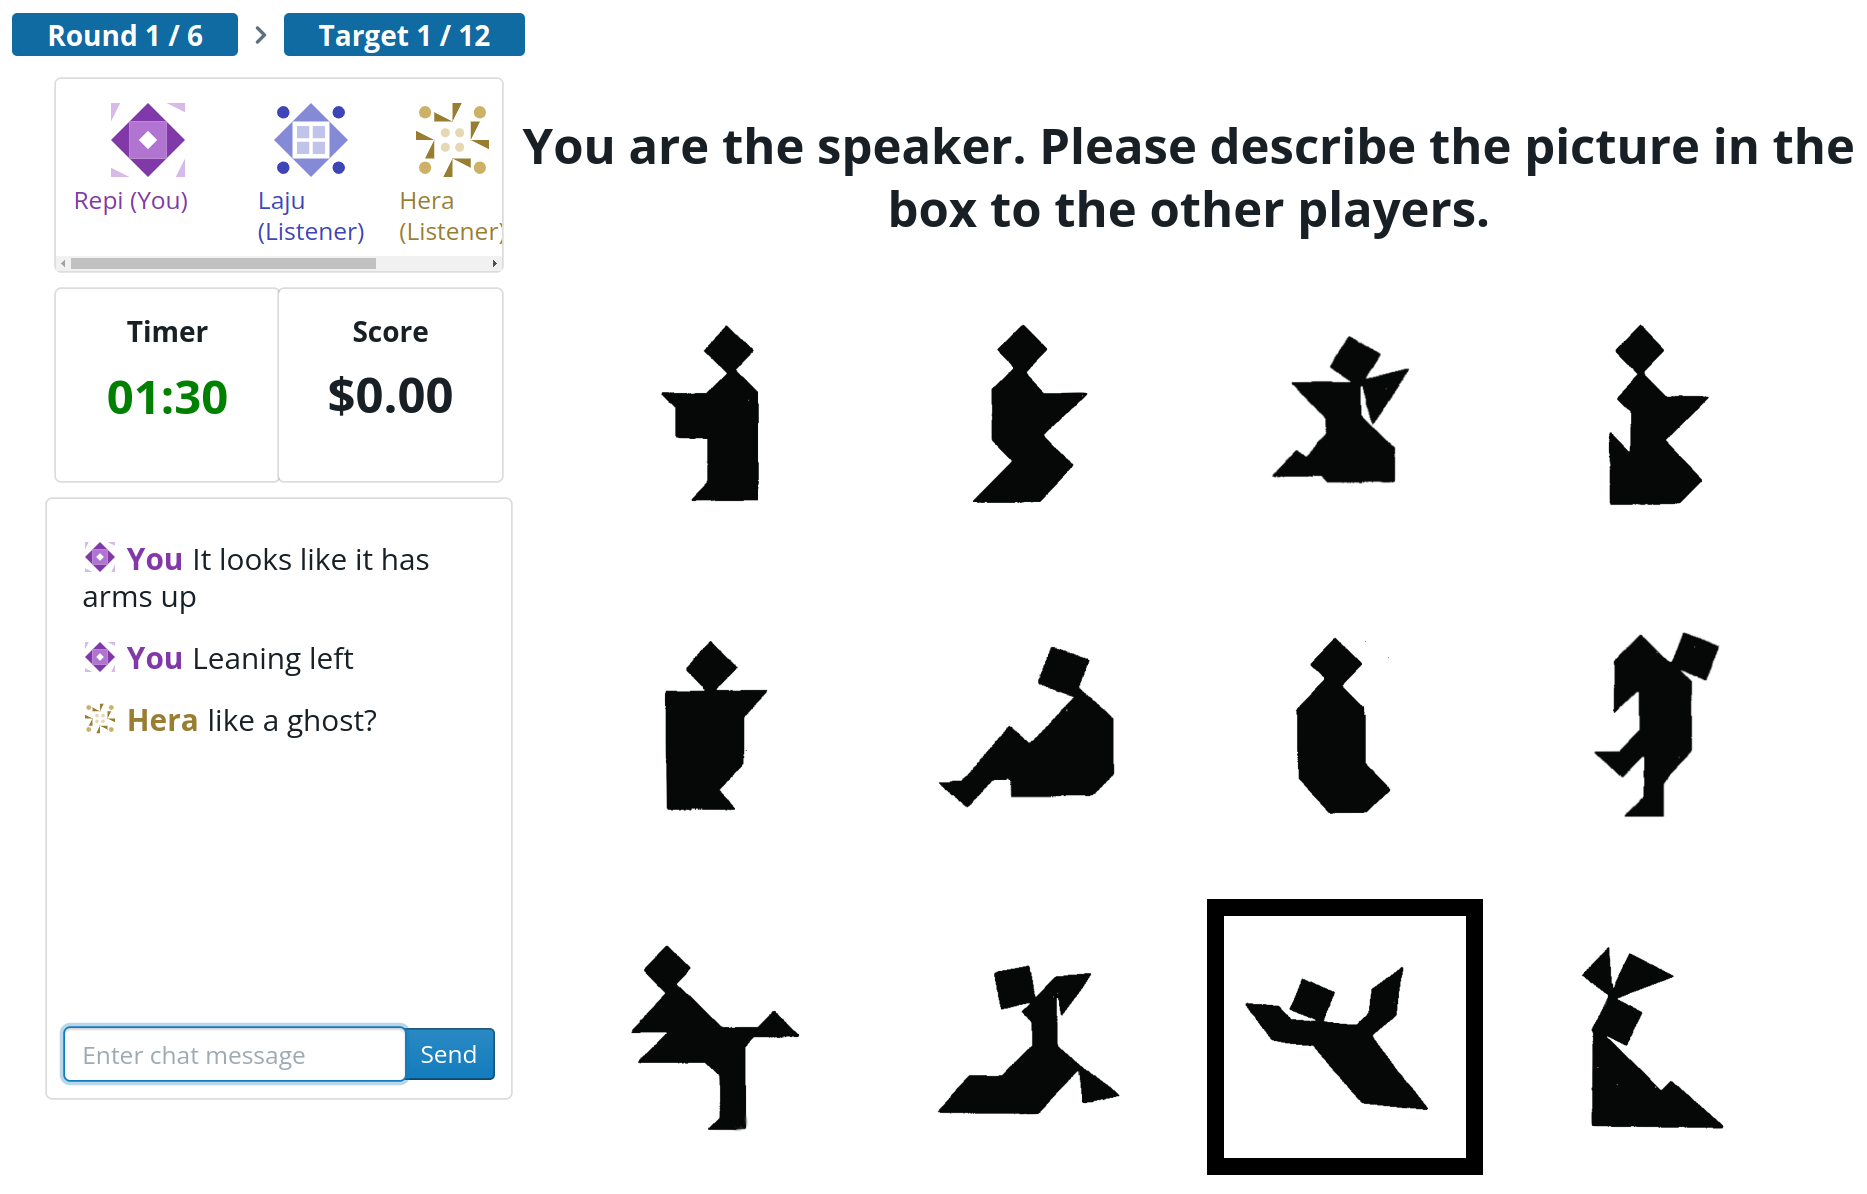
\includegraphics[width=20em]{images/diagram.png}};
		\node[anchor=north west] () at (11.5, 2.7) {Trial};
		
		\node[illus, anchor=north west, minimum width=25em, minimum height=18em] (block) at (7.5, 3) {};
		\node[anchor=north west] () at (11.5, 3.5) {Block};
		\node[anchor=north west] () at (14, -2.5) {x 12 images};
		\node[anchor=north west] () at (14, -3.3) {x 6 iterations};


	\node at (-4.5,-5.2) {\LARGE\bfseries{C}};
%	\node[bound, ultra thick, anchor=north, minimum width=50em, minimum height=17em] (block) at (6.5, -5.5) {};
		
	 \node[illus, anchor=east] () at (1.8,-10.3) {Emoji \\ 
\includegraphics[height=3.5em]{images/nochat.png}};
	 \node[align=center, anchor=center] at (2.5,-9) {Listener  Backchannel};
	\node[illus, anchor=west] () at (2,-10.3) {Chat \\ 
\includegraphics[height=3.5em]{images/chat.png}};

		\node[illus,anchor=east] () at (11.4,-10.3) {Two person \\ 
\includegraphics[height=3em]{images/two.png}};
			 \node[align=center, anchor=center] at (11.5,-9) {Group  size};
	\node[illus, anchor=west] () at (11.6,-10.3) {Six person \\ 
\includegraphics[height=3em]{images/six.png}};
	
	\node[illus, anchor=east] () at (2.4,-6.8) {Rotate speaker\\ 
\includegraphics[height=4em]{images/rotate.png}};
		 \node[align=center, anchor=center] at (2.5,-5.5) {Group  coherence:  Speaker rotation};
	\node[illus, anchor=west] () at (2.6,-6.8) {Consistent speaker\\ 
\includegraphics[height=4em]{images/norotate.png}};
	
	\node[illus, anchor=east] () at (11.4,-7) {Limited feedback\\ 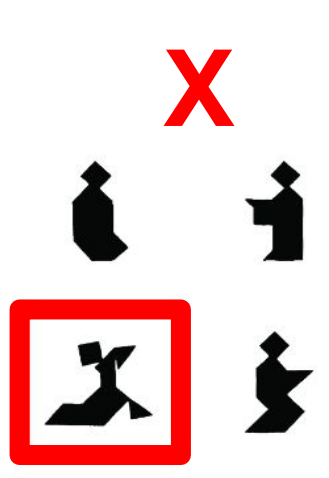
\includegraphics[height=5em]{images/limited-wrong.png} 
\phantom{m} 
\includegraphics[height=5em]{images/limited-correct.png}};
	\node[align=center, anchor=center] at (11.5,-5.5) {Group  coherence:  Feedback};
	\node[illus, anchor=west] () at (11.6,-7) {Full feedback \\  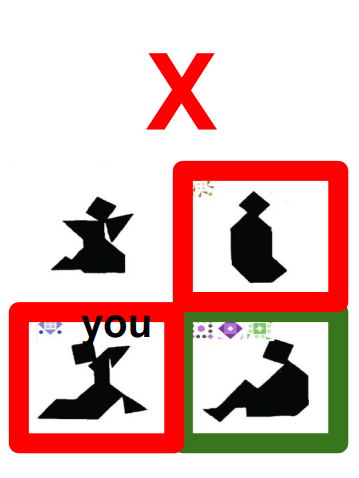
\includegraphics[height=5em]{images/full-wrong.png}  \phantom{m} 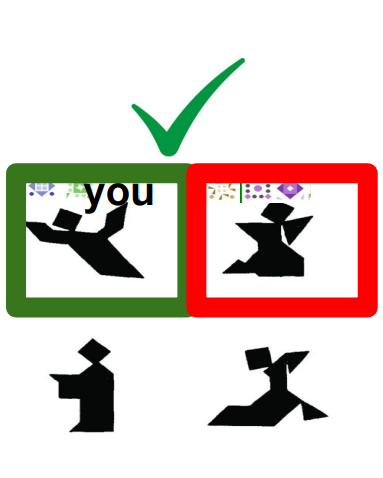
\includegraphics[height=5em]{images/full-correct.png}	};


		

		
		
		
	\end{tikzpicture}
	




	

\end{document}